% ieeeaccess.cls reuses \year as a metadata setter. Preserve the TeX primitive
% so PGF/TikZ can initialize its deterministic machinery while loading.
\let\PSevenTeXYear\year
\documentclass{ieeeaccess}

% Shared packages and notation. Do not change IEEE Access class formatting here.
\usepackage{cite}
\usepackage{amsmath,amssymb,amsfonts}
\usepackage{graphicx}
\usepackage{textcomp}
\usepackage{bm}
\usepackage{booktabs}
\usepackage{array}
\usepackage{tabularx}
\usepackage{xcolor}
% The legacy IEEE Access class encodes its blue as a Pantone spot color that
% some current PDF renderers drop. Preserve the journal hue in device RGB so
% titles, section heads, and captions remain visible in archival renderers.
\definecolor{accessblue}{RGB}{0,114,178}
\let\PSevenIEEEAccessYear\year
\let\year\PSevenTeXYear
\usepackage{tikz}
\let\year\PSevenIEEEAccessYear
\usetikzlibrary{arrows.meta,positioning,fit,calc,shapes.geometric,backgrounds}
\usepackage[hidelinks]{hyperref}
\usepackage{etoolbox}

% ieeeaccess.cls adds an unnumbered REFERENCES entry to the PDF outline after
% creating the heading. Supply its hyperlink destination without altering the
% official class or its visual bibliography formatting.
\makeatletter
\patchcmd{\thebibliography}{\section*{\refname}}{\section*{\refname}\phantomsection}{}{}
\makeatother

% Replace the class template's published-volume placeholder with an honest
% circulation marker. The official class file itself remains unmodified.
\newcommand{\PSevenDraftFooter}{PREPRINT}
\makeatletter
\patchcmd{\ps@titlepage}{\footervolfont VOLUME\ \thevol, \theyear}{\footervolfont\PSevenDraftFooter}{}{}
\patchcmd{\ps@titlepage}{\footervolfont VOLUME\ \thevol, \theyear}{\footervolfont\PSevenDraftFooter}{}{}
\patchcmd{\ps@headings}{\footervolfont VOLUME\ \thevol, \theyear}{\footervolfont\PSevenDraftFooter}{}{}
\patchcmd{\ps@headings}{\footervolfont VOLUME\ \thevol, \theyear}{\footervolfont\PSevenDraftFooter}{}{}
\AtBeginDocument{\ps@headings}
\makeatother

\newtheorem{proposition}{Proposition}
\newtheorem{definition}{Definition}
\newtheorem{corollary}{Corollary}

\DeclareMathOperator*{\argmax}{arg\,max}
\DeclareMathOperator*{\argmin}{arg\,min}
\newcommand{\R}{\mathbb{R}}
\newcommand{\Pset}{\mathcal{P}}
\newcommand{\Hset}{\mathcal{H}}
\newcommand{\given}{\,|\,}

% Writing-assistance attribution, separate from scientific-source citations.
\newcommand{\AIDraftingCredit}{\footnote{Drafting/revision assistance:
OpenAI Codex~\cite{openaiCodex2026}.}}

\usepackage{pdfpages}
\usepackage{placeins}
\newcommand{\ObservedPMUCount}{8}
\newcommand{\HiddenBusCount}{31}
\newcommand{\NominalTestCount}{100}
\newcommand{\BZeroTVE}{0.3402\%}
\newcommand{\BOneTVE}{0.009904\%}
\newcommand{\BTwoTVE}{0.009634\%}
\newcommand{\BTwoRelativeImprovement}{2.7\%}
\newcommand{\BTwoMinusBOnePP}{-0.000270}
\newcommand{\BTwoMinusBOneCILowPP}{-0.000359}
\newcommand{\BTwoMinusBOneCIHighPP}{-0.000179}
\newcommand{\BTwoWinRate}{69.0\%}
\newcommand{\FunctionalSpearman}{0.5625}
\newcommand{\FunctionalSpearmanCILow}{0.271}
\newcommand{\FunctionalSpearmanCIHigh}{0.751}
\newcommand{\FunctionalPermutationP}{0.0012}
\newcommand{\FunctionalKendall}{0.376}
\newcommand{\MismatchMainCount}{980}
\newcommand{\MismatchRefinementCount}{175}
\newcommand{\NetworkMismatchRatio}{16.99}
\newcommand{\OperatingMismatchRatio}{8.32}
\newcommand{\OnlineClosurePercent}{0.4\%}
\newcommand{\UtwoNLL}{-16.184}
\newcommand{\UtwoCoverageRe}{93.9\%}
\newcommand{\UtwoCoverageIm}{94.2\%}
\newcommand{\OriginalInnovationACF}{0.602}
\newcommand{\MeasurementGMInnovationACF}{0.540}
\newcommand{\MismatchUzeroCoverage}{92.9\%}
\newcommand{\MismatchUtwoCoverage}{47.5\%}
\newcommand{\AdequacyHalfAUROC}{0.901}
\newcommand{\AdequacyHalfAUPRC}{0.779}
\newcommand{\AdequacyMaxAUROC}{0.928}
\newcommand{\AdequacyMaxAUPRC}{0.787}
\newcommand{\NetworkFrozenTVE}{0.250430\%}
\newcommand{\NetworkOracleTVE}{0.002547\%}
\newcommand{\NetworkOnlineTVE}{0.251132\%}
\newcommand{\OperatingFrozenTVE}{0.122641\%}
\newcommand{\OperatingOracleTVE}{0.001006\%}
\newcommand{\OperatingOnlineTVE}{0.122381\%}
\newcommand{\CoupledFrozenTVE}{0.023615\%}
\newcommand{\CoupledOracleTVE}{0.000396\%}
\newcommand{\CoupledOnlineTVE}{0.023615\%}
\newcommand{\EZeroHDevCount}{30}
\newcommand{\EZeroHTestCount}{60}
\newcommand{\EZeroHValidRate}{100.0\%}
\newcommand{\EZeroHClosureOverall}{98.1\%}
\newcommand{\EZeroHRuntimeMedian}{61.7}
\newcommand{\EZeroHRuntimePNinetyFive}{76.0}
\newcommand{\EZeroHRank}{25}
\newcommand{\EZeroHDimension}{43}
\newcommand{\EZeroHNullity}{18}
\newcommand{\EZeroHFunctionalResidual}{0.0419}
\newcommand{\EZeroHFrozenHalf}{0.19885\%}
\newcommand{\EZeroHFrozenOne}{0.38834\%}
\newcommand{\EZeroHFrozenMax}{0.57795\%}
\newcommand{\EZeroHCorrectedHalf}{0.00525\%}
\newcommand{\EZeroHCorrectedOne}{0.00749\%}
\newcommand{\EZeroHCorrectedMax}{0.00974\%}
\newcommand{\EZeroHClosureHalf}{97.4\%}
\newcommand{\EZeroHClosureOne}{98.1\%}
\newcommand{\EZeroHClosureMax}{98.3\%}
\newcommand{\EZeroHNEESHalf}{111.6}
\newcommand{\EZeroHNEESOne}{183.3}
\newcommand{\EZeroHNEESMax}{294.2}
\newcommand{\LegacyEventTrajectories}{690}
\newcommand{\LegacyEventDetectionFOne}{0.989}
\newcommand{\LegacyEventMacroFOne}{0.905}
\newcommand{\LegacyPhysicalTopOne}{0.592}
\newcommand{\LegacyPhysicalTopThree}{0.719}
\newcommand{\LegacyIntegrityTopOne}{0.974}
\newcommand{\LegacyFalseAlarmsPerMinute}{1.45}
\newcommand{\LegacyPhysicalGainPP}{9.6}
\newcommand{\LegacyPhysicalGainCILowPP}{6.9}
\newcommand{\LegacyPhysicalGainCIHighPP}{12.5}
\newcommand{\HeldSourceCorrect}{3}
\newcommand{\HeldSourceDecisions}{303}
\newcommand{\HeldSourceCases}{101}
\newcommand{\HeldSourceRate}{1.0\%}
\newcommand{\RawCandidateEventEpisodes}{2.7}
\newcommand{\RawCandidatePhysicalEpisodes}{0.3}
\newcommand{\LoadSourceCount}{16}
\newcommand{\LoadTangentMaxRelError}{0.235\%}
\newcommand{\LoadTangentMinCosine}{0.999995}
\newcommand{\LoadTangentMedianStressError}{1.56\%}
\newcommand{\LoadTangentMaxStressError}{4.55\%}
\newcommand{\LoadVOneEventCases}{2560}
\newcommand{\LoadVOneNoEventCases}{320}
\newcommand{\LoadVOneFPR}{0.625\%}
\newcommand{\LoadVOneTopOne}{100.0\%}
\newcommand{\LoadWeakEventCases}{9600}
\newcommand{\LoadWeakNoEventCases}{800}
\newcommand{\LoadFiniteEventCases}{8000}
\newcommand{\LoadTruncationSlope}{2.00}
\newcommand{\LoadTruncationCILow}{1.79}
\newcommand{\LoadTruncationCIHigh}{2.24}
\newcommand{\LoadWTwoNIS}{0.998}
\newcommand{\LoadWTwoACFOne}{-0.0026}
\newcommand{\LoadWTwoLjungP}{0.598}
\newcommand{\LoadLTwoDevCoverage}{95.0\%}
\newcommand{\LoadEVIRho}{-0.794}
\newcommand{\LoadProjectedFisherRho}{0.361}
\newcommand{\LoadWeakMinAUROC}{0.731}
\newcommand{\LoadWeakMinTopOne}{12.8\%}
\newcommand{\LoadFiniteCoverageMin}{92.9\%}
\newcommand{\LoadFiniteCoverageMax}{96.0\%}
\newcommand{\GlobalHypothesisCount}{137}
\newcommand{\GlobalPhysicalTrajectories}{3488}
\newcommand{\GlobalNoiseRecords}{10564}
\newcommand{\GlobalEventRecords}{10564}
\newcommand{\GlobalEventAUROC}{0.990}
\newcommand{\GlobalEventAUPRC}{0.9999}
\newcommand{\GlobalEventFNR}{7.3\%}
\newcommand{\GlobalEventFPRUpper}{3.6\%}
\newcommand{\GlobalWeakCardinality}{37.4\%}
\newcommand{\GlobalWeakTopOne}{24.4\%}
\newcommand{\GlobalWeakTopThree}{59.8\%}
\newcommand{\GlobalWeakStrongTopOne}{66.2\%}
\newcommand{\GlobalModerateTopOne}{98.8\%}
\newcommand{\GlobalFiniteTopOne}{100.0\%}
\newcommand{\GlobalInclusionAUROC}{0.950}
\newcommand{\GlobalInclusionECE}{0.029}
\newcommand{\WeakGlobalExactRho}{0.780}
\newcommand{\WeakSupportOnlyExactRho}{0.140}
\newcommand{\TOneTwentyGammaFour}{2844.44}
\newcommand{\TOneTwentyInfoRatio}{8.37}
\newcommand{\TOneTwentyCompleteMedianError}{0.0031}
\newcommand{\TOneTwentyCompleteMedianEta}{5.36e-04}
\newcommand{\TOneTwentyCompleteMaxEta}{0.088}
\newcommand{\TOneTwentyDMedianError}{0.2053}
\newcommand{\TOneTwentyDQMedianError}{0.4690}
\newcommand{\TOneTwentyHardPairSigma}{225.3}
\newcommand{\TOneTwentyHardPairCoherence}{0.999976}
\newcommand{\TOneTwentySevenTwelveCoherence}{-0.997947}
\newcommand{\TOneTwentyRuntime}{5.446}

\newcommand{\ContMixTimely}{53}
\newcommand{\ContMixTotal}{54}
\newcommand{\ContMixExtras}{4}
\newcommand{\ContMixOutTimely}{17}
\newcommand{\ContMixBusTimely}{2}
\newcommand{\ContNomTimely}{54}
\newcommand{\ContNomTotal}{54}
\newcommand{\ContNomExtras}{7}
\newcommand{\ContNomOutTimely}{18}
\newcommand{\ContNomBusTimely}{3}
\newcommand{\ContAdmissionTimely}{52}
\newcommand{\ContAdmissionTotal}{54}
\newcommand{\ContAdmissionExtras}{0}
\newcommand{\ContAdmissionOutTimely}{16}
\newcommand{\ContAdmissionBusTimely}{2}
\newcommand{\ContETTimely}{27}
\newcommand{\ContETTotal}{54}
\newcommand{\ContETExtras}{3}
\newcommand{\ContETOutTimely}{9}
\newcommand{\ContETBusTimely}{0}
\newcommand{\ContPriorTimely}{54}
\newcommand{\ContPriorExtras}{6}
\newcommand{\ChenMatchedCorrect}{299}
\newcommand{\ChenMatchedTotal}{300}
\newcommand{\ChenMatchedEarly}{1}
\newcommand{\ChenNormalExposure}{100,000}

\newcommand{\NarMixDetected}{54}
\newcommand{\NarMixJoint}{54}
\newcommand{\NarMixTimely}{53}
\newcommand{\NarMixEvents}{54}
\newcommand{\NarMixLoadTimely}{26}
\newcommand{\NarMixLoadTotal}{27}
\newcommand{\NarMixLineTimely}{27}
\newcommand{\NarMixLineTotal}{27}
\newcommand{\NarMixExtras}{4}
\newcommand{\NarNomDetected}{54}
\newcommand{\NarNomJoint}{54}
\newcommand{\NarNomTimely}{54}
\newcommand{\NarNomEvents}{54}
\newcommand{\NarNomLoadTimely}{27}
\newcommand{\NarNomLoadTotal}{27}
\newcommand{\NarNomLineTimely}{27}
\newcommand{\NarNomLineTotal}{27}
\newcommand{\NarNomExtras}{7}
\newcommand{\NarETDetected}{27}
\newcommand{\NarETJoint}{27}
\newcommand{\NarETTimely}{27}
\newcommand{\NarETEvents}{54}
\newcommand{\NarETLoadTimely}{0}
\newcommand{\NarETLoadTotal}{27}
\newcommand{\NarETLineTimely}{27}
\newcommand{\NarETLineTotal}{27}
\newcommand{\NarETExtras}{3}
\newcommand{\NarETSDetected}{27}
\newcommand{\NarETSJoint}{27}
\newcommand{\NarETSTimely}{27}
\newcommand{\NarETSEvents}{54}
\newcommand{\NarETSLoadTimely}{0}
\newcommand{\NarETSLoadTotal}{27}
\newcommand{\NarETSLineTimely}{27}
\newcommand{\NarETSLineTotal}{27}
\newcommand{\NarETSExtras}{3}
\newcommand{\NarWitnessDetected}{53}
\newcommand{\NarWitnessJoint}{53}
\newcommand{\NarWitnessTimely}{52}
\newcommand{\NarWitnessEvents}{54}
\newcommand{\NarWitnessLoadTimely}{25}
\newcommand{\NarWitnessLoadTotal}{27}
\newcommand{\NarWitnessLineTimely}{27}
\newcommand{\NarWitnessLineTotal}{27}
\newcommand{\NarWitnessExtras}{0}

\IfFileExists{generated/c01_macros.tex}{\input{generated/c01_macros}}{}

\newcommand{\PSevenSupplementPDF}{output/pdf/P07_Physics_Informed_State_Reconstruction_Event_Source_Inference_Supplement.pdf}

\begin{document}
\history{}
\doi{}

\title{Physics-Based Event Attribution From Sparse PMUs With Recovery Memory}
\author{\uppercase{Jorge Luis Mayorga Taborda}\authorrefmark{1}, \uppercase{Yessica Africano Rodriguez}\authorrefmark{1}, \uppercase{Masoud Barati}\authorrefmark{2}, \uppercase{Payman Dehghanian}\authorrefmark{3}, AND \uppercase{David Felipe Celeita Rodr\'iguez}\authorrefmark{4}}

\address[1]{Universidad de los Andes, Bogot\'a, Colombia}
\address[2]{Department of Electrical and Computer Engineering, University of Pittsburgh, Pittsburgh, PA, USA}
\address[3]{Department of Electrical and Computer Engineering, The George Washington University, Washington, DC, USA}
\address[4]{Faculty of Engineering, Universidad de La Sabana, Ch\'ia, Colombia}
\corresp{Corresponding author: Jorge Luis Mayorga Taborda (e-mail: jl.mayorga236@uniandes.edu.co).}

\markboth{Mayorga Taborda \headeretal, Sparse-PMU Attribution With Recovery Memory}{Mayorga Taborda \headeretal, Sparse-PMU Attribution With Recovery Memory}

\hypersetup{
  pdftitle={Recovery-Aware Physical Event Attribution From Sparse PMUs},
  pdfauthor={Jorge Luis Mayorga Taborda; Yessica Africano Rodriguez; Masoud Barati; Payman Dehghanian; David Felipe Celeita Rodriguez},
  pdfsubject={Sparse-PMU state reconstruction, finite-horizon diagnosability, and multi-event source inference},
  pdfkeywords={dynamic state estimation, functional observability, phasor measurement units, physics-informed inference, source localization}
}

\begin{abstract}
Sparse PMUs can reveal a disturbance without identifying its physical source, especially when a new intervention begins during recovery from an earlier one. We study this ambiguity through competing intervention-conditioned network trajectories. A frozen differential-algebraic model predicts voltage, terminal current, frequency and ROCOF at eight PMUs. A causal history bank tests load and line hypotheses over a ten-second retrospective window, integrates load severity, retains the originating cause after restoration, and combines fixed network-model hypotheses. Its source masses $M$ and increments distinguish conditional evidence from model reweighting. Physical restoration changes the operator without erasing the state, so recovery remains a candidate explanation for subsequent measurements. Separate experiments expose the information limit: accurate hidden-voltage recovery does not imply source separation, and weak-pair exact-support Top-1 in the matched batch study is \GlobalWeakTopOne{}, versus \GlobalFiniteTopOne{} for finite pairs. In continuous-stream development tests, the bank obtains \ContMixTimely{}/\ContMixTotal{} timely family/source decisions with \ContMixExtras{} unmatched alarms. Nominal gains one timely decision at a higher alarm burden; stricter admission loses a real intervention. Confirmatory performance remains pending completion of the frozen campaign. The demonstrated scope is a known load/line catalog under stated network uncertainty, without a universal optimality or all-family claim.
\end{abstract}

\begin{keywords}
dynamic state estimation, event detection, functional observability, limited observability, phasor measurement units, physics-informed inference, source localization.
\end{keywords}

\titlepgskip=-21pt
\maketitle

\section{Introduction}
\label{sec:introduction}

\PARstart{A}{n} unmeasured load changes. Several PMUs respond, a detector raises an alarm, and the network keeps oscillating after the load is restored. A second intervention then begins during that recovery. The operational question is no longer whether one signal exceeds a threshold: which physical intervention explains the reports observed so far, where did it originate, and when is that explanation distinguishable from the alternatives?

\begin{figure*}[t]\centering
\resizebox{\textwidth}{!}{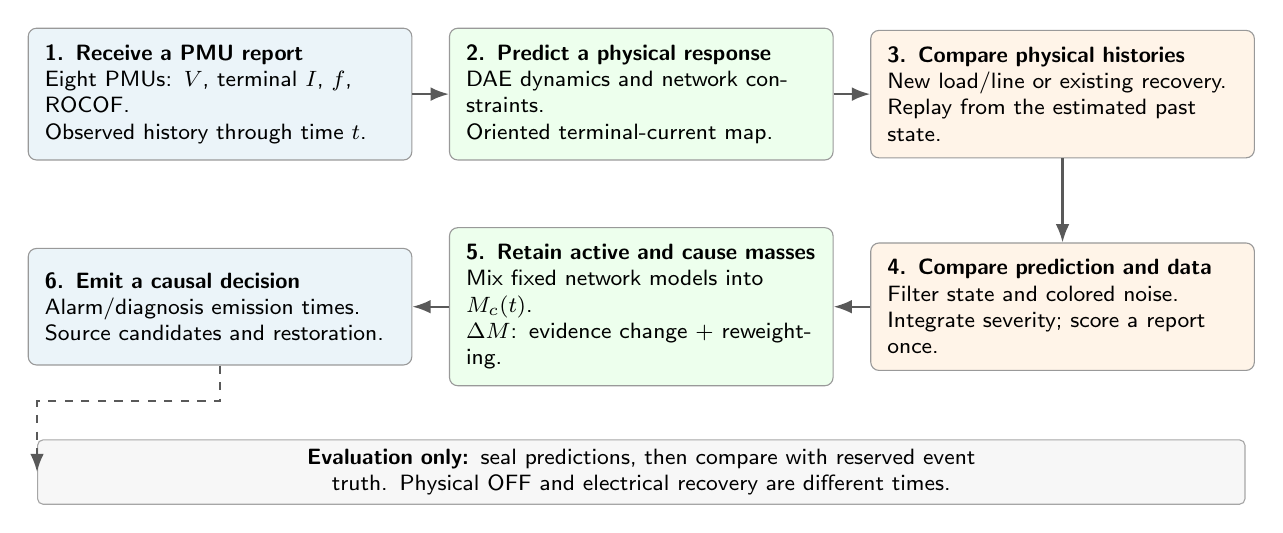
\begin{tikzpicture}[font=\sffamily\footnotesize\mdseries,>=Latex,
 box/.style={draw=black!40,rounded corners=3pt,align=left,text width=4.45cm,minimum height=1.48cm,inner sep=6pt},
 arr/.style={->,thick,draw=black!65}]
\node[box,fill=accessblue!8] (y) at (0,0) {\textbf{1. Receive a PMU report}\\Eight PMUs: $V$, terminal $I$, $f$, ROCOF.\\Observed history through time $t$.};
\node[box,fill=green!7] (physics) at (5.35,0) {\textbf{2. Predict a physical response}\\DAE dynamics and network constraints.\\Oriented terminal-current map.};
\node[box,fill=orange!9] (hyp) at (10.7,0) {\textbf{3. Compare physical histories}\\New load/line or existing recovery.\\Replay from the estimated past state.};
\node[box,fill=orange!9] (like) at (10.7,-2.7) {\textbf{4. Compare prediction and data}\\Filter state and colored noise.\\Integrate severity; score a report once.};
\node[box,fill=green!7] (mass) at (5.35,-2.7) {\textbf{5. Retain active and cause masses}\\Mix fixed network models into $M_c(t)$.\\$\Delta M$: evidence change + reweighting.};
\node[box,fill=accessblue!8] (out) at (0,-2.7) {\textbf{6. Emit a causal decision}\\Alarm/diagnosis emission times.\\Source candidates and restoration.};
\draw[arr] (y)--(physics);\draw[arr] (physics)--(hyp);\draw[arr] (hyp)--(like);\draw[arr] (like)--(mass);\draw[arr] (mass)--(out);
\node[draw=black!35,fill=black!3,rounded corners=2pt,align=center,text width=15.1cm,minimum height=.68cm] (eval) at (5.35,-4.8) {\textbf{Evaluation only:} seal predictions, then compare with reserved event truth. Physical OFF and electrical recovery are different times.};
\draw[arr,dashed] (out.south)--++(0,-.45)-|(eval.west);
\end{tikzpicture}
}
\caption{The complete scientific argument. Physics maps an intervention at an unmeasured source into predicted PMU trajectories; causal evidence chooses among those explanations. Event truth enters only evaluation. The figure describes the implemented restricted load/line component, not an already validated all-family joint estimator.}
\label{fig:joint-architecture}\end{figure*}

Sparse PMUs make the question difficult because a source need not have a sensor at its own bus. Its voltage, current and frequency effects propagate through the network \cite{phadke2008synchronized,zhao2019dse}. Uncertain operating context and network parameters can also change those effects. Moreover, physical OFF is not electrical recovery. A method that resets at restoration can treat the remaining response as another event or lose a real event that begins before the oscillation decays.

Strong existing methods solve parts of this problem. Dynamic state estimators combine power-system equations and PMU histories \cite{katanic2024recursive}; supervised classifiers learn sparse-PMU event/source labels \cite{pandey2020realtime,yildiz2024few}; physical outage detectors compare network hypotheses sequentially \cite{chen2016quickest,rovatsos2017outage}; and high-fidelity fault trajectories already support sparse-PMU diagnosis \cite{warner2023highfidelity}. The question here is how to retain an explanation through restoration and compare its recovery with a later intervention. A low state error does not prove source identity, and a score on represented assets does not prove source transfer.

Our approach uses the physical intervention as the object of inference. A load or line candidate changes the network's DAE operator. Starting from an estimated past state, that operator predicts what all eight PMUs should report. Conditional likelihoods compare those responses with the observed history while retaining amplitude, noise and network-model uncertainty. The source/family masses $M$ summarize the competing explanations; their increments separate conditional evidence evolution from reweighting physical models. Retained recovery states compete against new events rather than being discarded at OFF.

The paper makes three scoped contributions:
\begin{enumerate}
\item \textbf{Recovery-aware physical attribution:} an executable causal load/line history bank starts from estimated past states, retains the originating cause after physical OFF, and compares recovery with new-intervention histories under fixed network hypotheses. We specify its evidence and publication rules.
\item \textbf{A bounded source-resolution analysis:} applying established observability and diagnosability ideas, the matched load-support study distinguishes accurate state reconstruction from reliable source identity and exposes weak-source ambiguity. This is a separate component test, not a causal optimality theorem.
\item \textbf{A reproducible operational test:} the nominal/mixture comparison and a failed admission ablation expose the trade-off between timely source attribution and extra alarms. Separate state, batch and stream contracts retain their own denominators. R11 and nominal remain frozen co-references for confirmation.
\end{enumerate}

The methodological contribution is the specified competition between intervention and recovery histories under the declared sparse-PMU contract. Physical templates, retrospective onset search, standard Bayesian updates and the array name are established or elementary ingredients. We claim neither their first use nor a globally optimal filter. In completed development evidence, the five-model bank obtains \ContMixTimely{}/\ContMixTotal{} timely family/source decisions with \ContMixExtras{} extras; nominal retains one more timely event at a higher alarm burden. These tests support a restricted capability, not numerical superiority over every cited method. Final performance claims require the separate frozen confirmation.



\section{Closest Methods and the Remaining Question}
\label{sec:narrative-related}

Dynamic state estimation supplies the state and uncertainty machinery used to predict a PMU history. Unknown-input and DAE estimators address incomplete models and exogenous inputs \cite{gillijns2007input,nugroho2022dae,katanic2024recursive}. Their task is not automatically an event-family/source decision. A recovered bus-voltage field can remain compatible with competing physical interventions.

Model-based source inference is the closest methodological precedent. Phasor angles support outage hypotheses \cite{tate2008outage}; uncertain pre-event conditions can be marginalized with outage identity \cite{zhao2014outages}; and sequential likelihoods detect line changes under stochastic operation \cite{chen2016quickest,rovatsos2017outage}. Transient dynamics and unknown onset are therefore established ingredients, not contributions of this paper.

Warner \emph{et al.} provide a particularly close precedent \cite{warner2023highfidelity}. Their simulated voltage/current fault trajectories are compared with a steady-state reference over a moving onset window; Algorithm~1 stops and returns candidate lines. Load changes are an adverse-event test rather than a load-source output. Their Sections~II and IV target short-circuit identification before clearing, whereas our restricted task follows load changes and line openings through restoration and later interventions. Sparse sensing, a physical trajectory library and retrospective onset scanning are shared ideas. We have not run their procedure on the present data and make no numerical superiority claim over it.

Sequential diagnosis also has a stronger statistical literature than a rolling-window label suggests. The Adaptive Matrix CuSum addresses misidentification caused by pre-change observations and establishes delay/error results under its specified observation laws \cite{warner2024matrix}. R11's pruned conditional histories, colored measurement state and plug-in startup estimates do not inherit those guarantees. A ten-second window or the array $M$ is not a replacement for that theory.

Learned PMU diagnosis provides a different comparator. Sparse classifiers and knowledge-driven representations identify represented events or assets \cite{pandey2020realtime,li2024knowledge,yildiz2024few}. The historical SGSMA baseline supplies two frozen ExtraTrees adaptations here. We distinguish interpolation at represented sources, transfer of that frozen adapter, and true held-source generalization. The present causal catalog is known; its results do not establish the last of those claims.

Observability and diagnosability explain why neither a physical nor learned method is guaranteed to localize every visible event. Functional observability concerns the requested state function \cite{fernando2010functional,montanari2022functional}; descriptor-model diagnosability and nuisance-profiled tests concern competing explanations \cite{eriksson2013diagnosability,scharf1994matched}. Placement-dependent source ambiguity is also established in PMU fault/event work \cite{jamei2020limits,conte2023fault,yildiz2025sparse}. Our state/source distinction applies these ideas; it is not their first discovery.

Multiple-model filtering already manages conditional state/mode hypotheses \cite{blom1988imm}; R11 is a pruned history bank, not a new IMM derivation. Stochastic swing/kernel models estimate latent states in Ensaf and Barati \cite{ensaf2023kernel}, and physics-derived prior covariances support sparse-state forecasting \cite{tartakovsky2023gp}. Joint DAE-aware generator/network parameter inference is studied separately \cite{albustami2026dae}. R11 uses a finite bank of constant network hypotheses rather than inferring the continuous parameter posterior. A Gaussian process or neural architecture would require separate validation.

\begin{table*}[t]\centering\small
\caption{Closest inference contracts and the difference tested here. This is a methodological comparison; only Chen and the frozen ExtraTrees adapters are executed comparators in C01. Absence from a paper's evaluated task is not a claim of algorithmic impossibility.}\label{tab:literature-capability}
\begin{tabularx}{\textwidth}{@{}lXXX@{}}\toprule
Route & Physical/statistical mechanism & Published target & Difference or role here\\\midrule
Chen / Rovatsos & Increment statistics, network models and sequential tests & Line outages; Rovatsos includes transient phases & Chen is executed on persistent-line first stops\\
Warner high-fidelity & Simulated V/I paths, moving onset window, distance evidence & Short-circuit line candidates & Nearest trajectory precedent; no common-data run here\\
Adaptive Matrix CuSum & Pairwise sequential diagnosis and error/delay analysis & One unknown change among distributional alternatives & No corresponding optimality guarantee is claimed here\\
DAE / stochastic-state estimation & Incomplete DAE observers or physical uncertainty models & States, unknown inputs or network parameters & Components/adjacent tasks, not episode attribution scores\\
Knowledge-driven learned diagnosis & Spatiotemporal representation with topology/type constraints & Multi-family disturbance location & Distinct from the physical likelihood; ExtraTrees is our executed learned reference\\
Physical history bank here & Estimated-past-state paths, active/cause masses, fixed R/X mixture & Successive known-catalog load/line interventions & Test whether recovery-aware attribution retains timely sources without excess alarms\\\bottomrule
\end{tabularx}\end{table*}

The remaining question is operational and falsifiable: can a state-conditioned bank distinguish a new intervention from a preceding intervention's recovery while retaining timely family/source decisions under fixed network uncertainty? Our contribution is the specified recovery-aware construction and its bounded evidence, not a claim to have invented model-based diagnosis. We use ``physics-informed'' because physical equations define candidate trajectories and likelihood inputs. Learned discrepancy and the unrestricted joint state/event/integrity estimator remain separate proposals.

\section{The Decision Required From Eight PMUs}
\label{sec:narrative-problem}

At every report, the task is to decide whether the recent trajectory contains a physical intervention and, if so, identify its family, source and onset. Detection is the existence decision; classification chooses the physical operator; localization chooses a bus or branch. Those outputs need not become reliable at the same time. We keep the estimated physical onset $\widehat\tau$ separate from the time at which an alarm or diagnosis is emitted.

The network has 39 buses, but the prescribed PMU set is
\begin{equation}
 \mathcal P=\{2,5,6,10,19,22,29,39\}.
 \label{eq:narrative-pmus}
\end{equation}
Voltage is measured at each PMU bus. Current is measured at a specified branch terminal, which can differ from that bus. The causal implementation uses 47 coordinates: eight voltage magnitudes, eight voltage angles, eight current magnitudes, seven current angles, eight absolute frequencies and eight ROCOFs, at 30 reports/s. BUS39 current angle is excluded because its interpretation remains partially validated. The BUS5 current terminal retains the provisional historical 5--6 assignment. These are declared measurement assumptions, not identities inferred from classification accuracy.

\begin{figure*}[t]\centering
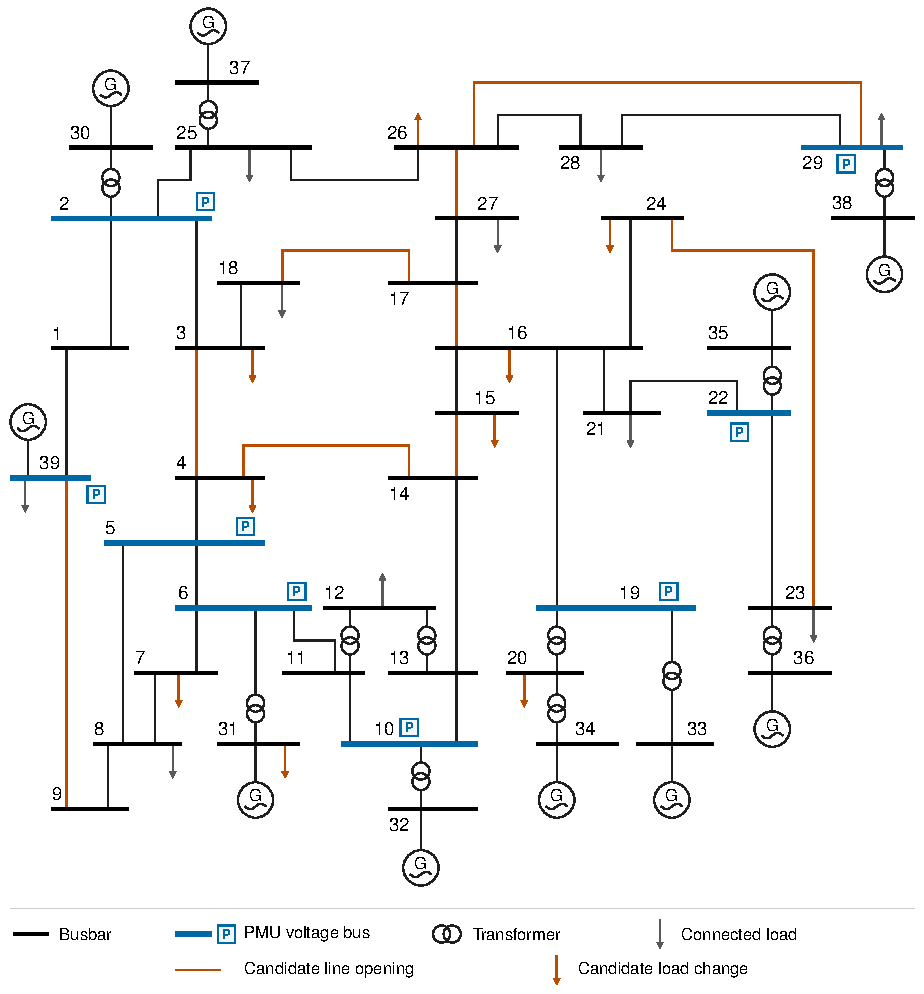
\includegraphics[width=.92\textwidth]{figures/generated/narrative_topology.pdf}
\caption{What is measured and what is hypothesized. The frozen causal bank contains nine load buses and nine line assets within the 39-bus network; eight blue buses carry PMUs. An unmeasured candidate is inferred through its network response at those PMUs. Orange branches are candidate interventions, not current-sensor assignments. Coordinates are schematic and do not define electrical distance.}
\label{fig:narrative-topology}\end{figure*}

The physical model is
\begin{align}
 \dot x&=f_q(x,z,u;\theta),&0&=g_q(x,z,u;\theta),\label{eq:narrative-dae}\\
 y_k&=\mathcal M_q(x_k,z_k;\theta_M)+b+\varepsilon_k.\label{eq:narrative-measurement}
\end{align}
Here $x$ contains machine and control dynamics, $z$ the algebraic network variables, $q$ the topology/intervention mode, and $\theta_M$ the measurement convention. The measurement map includes gains, phase references, orientation and the causal frequency/ROCOF estimator. A machine's rotor speed is not substituted for bus frequency.

An intervention hypothesis is $h=(e,c,\tau,a,d)$: family, source, onset, severity and duration. A load changes its local P/Q setpoints. A line opening switches its branch primitive; it is not approximated as a load change. For the supported impulse-free switches,
\begin{equation}
 x(\tau^+)=x(\tau^-),\qquad g_{q^+}(x(\tau^-),z(\tau^+),u;\theta)=0.
 \label{eq:narrative-switch}
\end{equation}
The algebraic voltage/current response may jump even though dynamic states remain continuous. Physical restoration reverses the intervention operator. It does not return the machines to their pre-event state, so electrical recovery can continue after OFF.

\begin{table}[t]\centering\small
\caption{Scope of the executed causal component. The source is an intervention asset; it is not necessarily a measured PMU bus.}\label{tab:narrative-scope}
\begin{tabularx}{\columnwidth}{@{}lXX@{}}\toprule
Case & Physical operator & Executed claim\\\midrule
Normal & No intervention & Monitor after startup\\
Load & Local P/Q factor; optional restoration & Nine candidate buses\\
Line & Branch open; optional reclose & Nine candidate branches\\
Fault/generation & Different shunt/input/trip operators & Outside this causal test\\
Missing/bad data & Measurement-integrity mechanism & Outside C01\\
Unknown & Unresolved diagnosis & Not a new physical family\\\bottomrule
\end{tabularx}\end{table}

The generator stores event schedules and true states separately from the PMU stream. Inference receives the nominal network, permitted calibration and reports through the current time. It receives no source, switch time, true R/X realization or solver state. Initial operating context and noise scale are estimated from 300 startup reports; monitoring begins after the inherited 12-s warmup. The startup contract assumes no intervention in that prefix.

\section{From Physical Predictions to Causal Attribution}
\label{sec:narrative-method}

\subsection{Where Physics Enters the Estimator}

The causal bank is the frozen R11 research implementation. Physics determines the candidate response, rather than supplying a penalty to a learned bus-label classifier. Kirchhoff constraints connect each unmeasured source to all available PMUs. With complex bus voltage $V$, the relevant electrical maps include
\begin{equation}
 I_{\rm bus}=Y_{\rm bus}V,\quad I_{{\rm term},r}=Y_{{\rm term},r}V,\quad
 S_i=V_i I_{{\rm bus},i}^{*}.
 \label{eq:narrative-electrical}
\end{equation}
Terminal-current rows retain transformer ratios, charging and orientation. A terminal current is not the bus injection in the power equation. A line hypothesis changes both the network constraints and the resulting terminal observations; a load hypothesis changes the local input and its dynamic propagation.

On a regular index-one DAE chart, differentiating the algebraic constraint gives the local predictor
\begin{align}
 \delta z&=-g_z^{-1}(g_x\delta x+g_u\delta u),\nonumber\\
 \delta\dot x&=(f_x-f_zg_z^{-1}g_x)\delta x
 +(f_u-f_zg_z^{-1}g_u)\delta u.
 \label{eq:narrative-reduction}
\end{align}
The frozen implementation builds transition/observation operators from the full DAE derivatives, with native terminal-current dependence for each topology. Equation~\eqref{eq:narrative-reduction} explains why an input at an unmeasured bus leaves a network-wide signature. It also explains why a local magnitude threshold alone cannot identify the source. Generator inertia, controls and the load law remain those of the frozen plant; no event-specific plant recalibration occurs here.

\subsection{Ask What Could Have Happened in the Last Ten Seconds}

At report time $t$, screening considers candidate onsets in $[t-10\,\mathrm{s},t]$. For each source and family it asks: if this intervention began at $\tau$, what reports should have arrived from $\tau$ to $t$? Prediction starts from the stored no-event state estimate at $\tau$, not a reset to nominal equilibrium. This matters when a new intervention arrives during recovery from the preceding one.

For a candidate history, the comparison is between a physical prediction and the same observed window,
\begin{align}
 r_{h,W}&=y_W-\widehat y_{h,W},\nonumber\\
 L_{h,W}&=\int p(y_W\mid h,a,\mathcal F_{\tau^-})p(a\mid h,\mathcal F_{\tau^-})\,da.
 \label{eq:narrative-evidence}
\end{align}
Conditional state filtering accounts for the retained physical state and colored instrumental noise. Load amplitude is integrated through the inherited truncated-Gaussian calculation; opening a line uses a switched operator. A finite line-screening response proposes a candidate, and the full switched operator confirms it from the estimated initial state. The rolling screen proposes useful histories; it is not additional independent evidence. A selected suffix is replayed with its original state snapshot, while the sequential likelihood scores each report once.

Supplementary Appendix~I gives the scalar precision/mean update and normalizing integral used for a retained load history. It makes the calculation reproducible without presenting standard Gaussian square completion as a new inference theorem.

\begin{figure*}[t]\centering
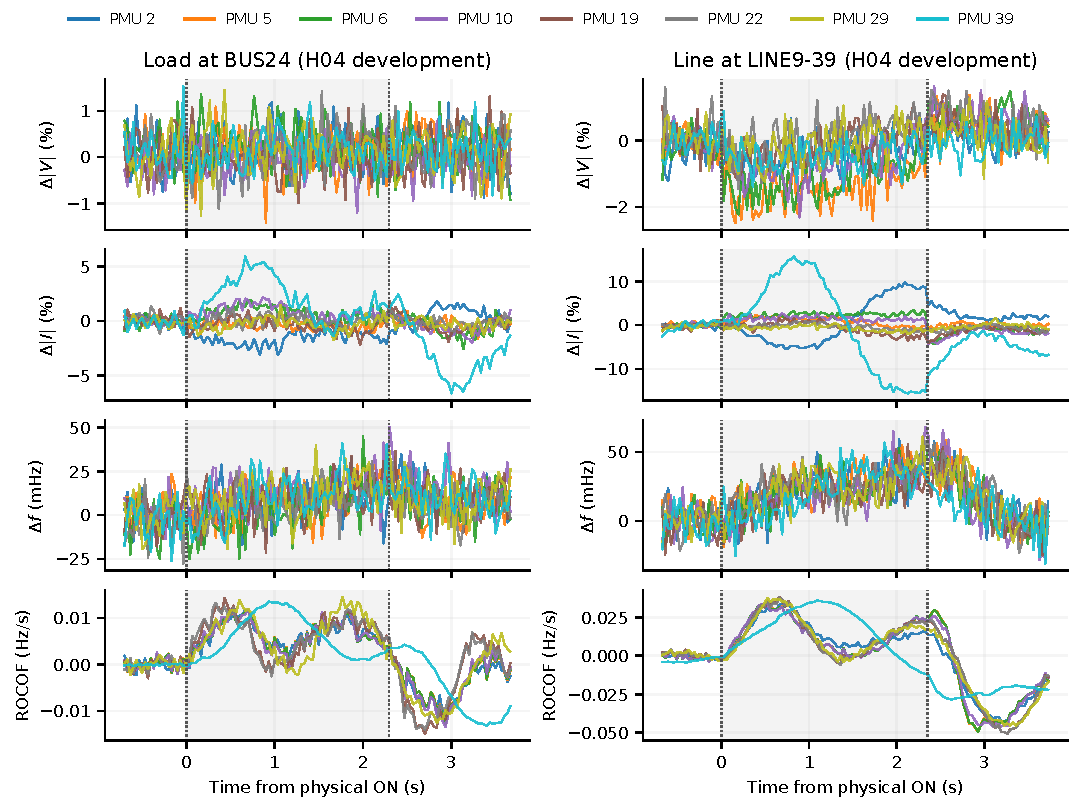
\includegraphics[width=.96\textwidth]{figures/generated/narrative_signals.pdf}
\caption{Why the method compares network responses. Two fixed H04 development examples show the first load and first line intervention in parent H002, measured at all eight PMUs. Shading marks the true intervention interval for retrospective explanation only. The different V/I/frequency/ROCOF responses are observations, not universal family templates: source, operating point and severity also change their shape. Frequency and ROCOF include the frozen causal instrumental estimator.}
\label{fig:narrative-signals}\end{figure*}

\subsection{Keep Reference Error Separate From Event Dynamics}

A wrong observation center can make a quiet network look disturbed. For each fixed network hypothesis $\theta_\ell$, startup estimates
\begin{equation}
 \widehat b_\ell=\overline y_{0:299}-y^{\rm ref}_\ell,
 \qquad b_{\ell,k}=\widehat b_\ell\quad(k\geq300).
 \label{eq:continuous-intercept}
\end{equation}
Angular differences use the common reference consistently. Frequency and ROCOF already have empirical startup centers and receive no extra intercept. The intercept is then frozen: it cannot follow a later load step and erase its signature. This is an observation-discrepancy correction, not recovery of the true impedances or a substitute for an AC-feasible hidden-state estimate. Its uncertainty and the operating-point estimate are treated by substitution.

The preservation mechanism is elementary but useful. For a fixed center, $T_b(y)=y-y^{\rm ref}-b$ satisfies $T_b(y+s)-T_b(y)=s$: a physical response $s$ is not projected away. Updating that center during an intervention would not retain this guarantee. Freezing the center preserves signatures; it does not repair wrong dynamic sensitivities.

Five constant network hypotheses represent nominal, global $\pm2\%$, and selected-branch $\pm3\%$ paired R/X changes. Each propagates its own conditional histories. The outer weight uses a predictive density formed before the current-report state update or screening:
\begin{equation}
 w_{\ell,k}=\frac{w_{\ell,k-1}p_\ell(y_k\mid\mathcal F_{k-1},\widehat b_\ell)}
 {\sum_jw_{j,k-1}p_j(y_k\mid\mathcal F_{k-1},\widehat b_j)}.
 \label{eq:continuous-weights}
\end{equation}
Startup reports are not scored again for network-model selection. Pruning, shared covariance approximations and adaptive history proposals make the result an approximate prequential mixture. We do not claim an optimal Kalman filter, a calibrated event posterior or identification of all line parameters.

\subsection{What $M$ and $\Delta M$ Actually Do}

Let $c$ index an admissible family/source cell. For a bus load the physical index is diagonal, $(i,i,\mathrm{load})$; for a line it is $(i,j,\mathrm{line})$. The implementation stores only the 18 allowed cells. It does not infer every event at every one of the 39 buses.

For network model $\ell$, let $M_{\ell,c,k}$ be the active history mass assigned to cell $c$. The mixed array and its exact increment are
\begin{align}
 M_{c,k}&=\sum_\ell w_{\ell,k}M_{\ell,c,k},\nonumber\\
 \Delta M_{c,k}&=\underbrace{\sum_\ell w_{\ell,k}(M_{\ell,c,k}-M_{\ell,c,k-1})}_{\text{conditional evidence evolution}}\nonumber\\
 &\quad+\underbrace{\sum_\ell(w_{\ell,k}-w_{\ell,k-1})M_{\ell,c,k-1}}_{\text{network-model reweighting}}.
 \label{eq:continuous-delta}
\end{align}
The array is operational: the mixed masses drive decisions. The decomposition identifies whether an attribution changed within the conditional observers or because network hypotheses were reweighted. It is an accounting identity checked by the code, not a new tensor-factorization theorem. A separate cause mass retains the originating intervention after it switches OFF, so the observer can explain recovery without declaring a new event.

The nominal reference runs the same physical/measurement construction with one network hypothesis and its own publication path. Comparing it with the five-model version tests the value and cost of model uncertainty without changing the plant or its source catalog.

\subsection{Why Restoration Does Not Remove the Physical Explanation}
\label{sec:recovery-mechanism}

Let $\kappa$ be a candidate restoration time. For the supported load and line
operators, the differential state is continuous even though the algebraic
solution can jump: $x(\kappa^+)=x(\kappa^-)$. Restoring the input or topology
therefore does not restore the pre-event state. On a regular, locally linear
post-restoration chart, compare the restored candidate with the same-context
no-new-intervention trajectory. Their state/output differences satisfy
\begin{align}
 \delta x_h(t)&\simeq\Phi_0(t,\kappa)\delta x_h(\kappa),\nonumber\\
 \delta q_h(t)&\simeq C_0(t)\Phi_0(t,\kappa)\delta x_h(\kappa),
 \quad t>\kappa,
 \label{eq:recovery-response}
\end{align}
where $q$ denotes the network voltage/terminal-current coordinates before
the frozen instrumental map. $\Phi_0$ propagates the restored DAE's reduced
dynamics and $C_0$ is its reduced observation map. The actual likelihood
also retains the measurement/filter memory. Thus the baseline during
recovery is a predicted trajectory, not a constant or zero residual.

Equation~\eqref{eq:recovery-response} is a local interpretation of retained
state propagation, not a new propagation law or an additional fitted model.
R11 keeps active-event mass separately from originating-cause mass. A new
intervention must compete with the existing recovery explanation; its
onset does not justify resetting either machine or instrumental states.
The H04 time trace illustrates this construction. The nominal comparison
isolates the outer network bank, while the admission ablation changes a
publication decision; neither alone isolates the causal benefit of every
recovery-state operation.

\subsection{Emit Decisions Without Resetting the Network}

An alarm, a confirmed family/source diagnosis and an estimated restoration are separate messages. The inherited configuration uses alarm/restoration mass thresholds of 0.99, six confirmation reports for alarm evidence, and 15 reports for restoration confirmation. These numbers are frozen method settings, not calibration guarantees. Additional source/line confirmation and episode-replacement rules remain those of the archived implementation; the configuration is included in the evidence snapshot.

Every emitted message records the latest report used. The observer continues through OFF with its conditional state and covariance; it does not reset to an equilibrium. A later event can begin while the network is still recovering. A source diagnosis emitted after true OFF remains correct eventually but fails the timely-localization metric.

The restricted runtime algorithm is: initialize from the permitted prefix; predict each fixed-model history; score the new report; propose/replay retrospective interventions when supported; mix the history masses; publish a confirmed decision; retain states through restoration. This is model-based Bayesian hypothesis inference. The ExtraTrees comparators are the learned components in this comparison; R11 has no learned bus-label head.

\FloatBarrier
\section{When a Physical Explanation Can Be Distinguished}
\label{sec:narrative-information}

A physical model does not remove an information limit. Two sources can produce nearly the same reports after their amplitudes and initial conditions are allowed to vary. High confidence in the state estimate therefore need not imply high confidence in a source.

The distinction is explicit in a local model. With observation matrix $C$, transition $A$ and requested hidden-voltage map $L$, functional reconstruction requires
\begin{equation}
 \ker\mathcal O_H\subseteq\ker L,\qquad
 \mathcal O_H=\operatorname{col}(C,CA,\ldots,CA^H).
 \label{eq:narrative-functional}
\end{equation}
Unobservable directions are harmless for this target if they do not change $Lx$ \cite{fernando2010functional,montanari2022functional}. Source attribution asks a stronger and different question. Let $s_i(\eta_i)$ and $s_j(\eta_j)$ be candidate trajectories after permitting their nuisance coordinates $\eta$, including severity and the admitted initial-state variation. Their profiled separation is
\begin{equation}
 D_{ij}(H)=\frac12\min_{\eta_i,\eta_j}
 \|s_i(\eta_i)-s_j(\eta_j)\|_{R_H^{-1}}^2.
 \label{eq:narrative-separation}
\end{equation}
Under a common Gaussian observation law, an intersection gives identical measurement distributions at that intersection. No classifier can then distinguish the candidates uniformly over the allowed nuisance set. A small positive distance can still leave a difficult, noise-sensitive decision \cite{eriksson2013diagnosability,scharf1994matched}. The detailed finite-horizon, signed-support and physical-boundary qualifications remain in Supplementary Appendix~D.

These are local conditions, not a structural certificate for the tested IEEE-39 configuration. The archived thresholded Gramian audit has a nonmonotone pseudo-rank and cannot supply that certificate. The nonlinear state-recovery result is evaluated independently; accurate target reconstruction is not used to claim full-state observability.

This framework explains the role of longer history: it may separate response paths that are close in one snapshot, but cannot guarantee an easy decision for every source and severity. It also explains why the estimator must keep competing hypotheses rather than turn every detected change into a confident location.

We test this mechanism with the separate batch reference $\mathcal E_{\mathrm B}$. It receives 32 rectangular voltage/current coordinates and is given the onset, load family and operating point; it compares 137 zero-, one- and two-source load supports and retains the original GH31 amplitude integration and W2 covariance. It is not R11 with a different solver, and R11 is not silently declared the complete joint estimator $\mathcal E_{\mathrm J}$. The batch study isolates source ambiguity; the causal study tests sequential decisions under a different contract.

\begin{figure*}[t]\centering
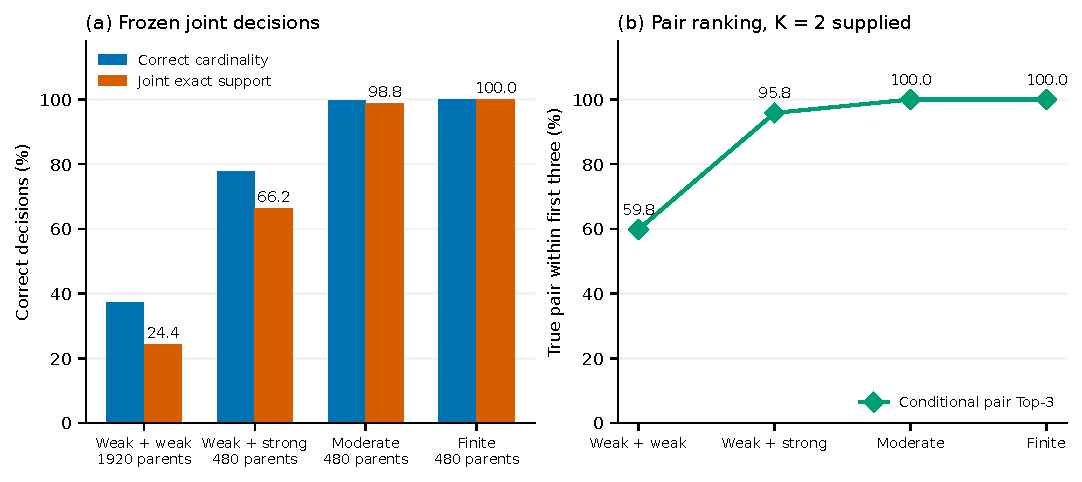
\includegraphics[width=.93\textwidth]{figures/generated/narrative_resolution.pdf}
\caption{The resolution limit behind the attribution problem. The frozen 137-hypothesis load bank increasingly recovers both cardinality and exact support as event strength increases. Weak-pair exact-support Top-1 is much lower than finite-pair Top-1. Cardinality means choosing the correct number of sources; support means choosing their identities. These known-onset batch results explain ambiguity and do not certify R11's causal performance. Repeated noise decisions are grouped by physical trajectory in the archived protocol.}
\label{fig:narrative-resolution}\end{figure*}

\section{Evidence Design and Fair Comparisons}
\label{sec:narrative-protocol}

The experiments answer three successive questions: does the physical model recover useful electrical information; are source responses distinguishable after nuisance fitting; and does a causal decision retain precision when interventions and recovery follow one another? They are separate tests, not parts of one pooled accuracy score.

\begin{table*}[t]\centering\small
\caption{One argument, distinct evidence contracts. An event realization repeats a physical parent under a condition or noise draw; it is not another independent physical event.}\label{tab:narrative-evidence}
\begin{tabularx}{\textwidth}{@{}lXXX@{}}\toprule
Question & Executed experiment & Decisive outcome & What it does not establish\\\midrule
Useful state information? & Separate B0--B3 voltage reconstruction and AC recentering & Hidden-voltage error and model-shift sensitivity & Source identity or calibrated joint covariance\\
Which sources are distinguishable? & Prospective 137-support batch load bank; known onset & Cardinality and exact-support recovery by severity & Unknown-onset multi-family monitoring\\
Can it monitor successive events? & H03/H04 continuous load/line development & Timely family/source, extras and restoration behavior & Confirmatory superiority or unseen-source transfer\\
Does the frozen result persist? & C01 configuration sealed before its new predictions & Independent-parent, paired R/X/noise comparison & No result is claimed until execution completes\\\bottomrule
\end{tabularx}\end{table*}

The causal simulator uses the frozen IEEE-39 Julia/PowerDynamics candidate, with continuous states and a separate PMU reporting grid. A 120-s record contains 3601 reports per PMU; a 600-s normal record contains 18001. Event-aligned reports use the consistent post-switch algebraic value, and solver diagnostics are stored separately. The measurement references, load law and stochastic instrument parameters are not retuned to individual events. RAW0001 is retrospective calibration evidence; RAW0002 remains unopened.

H03 and H04 each contain three event parents with six successive load/line interventions and one normal parent, all 80 s long. Schedules are paired across nominal, in-bank R/X and mixed out-of-bank R/X conditions. Each campaign therefore has 18 unique interventions and 54 event realizations. Both campaigns are now development evidence. No interval or generalization claim treats those 54 realizations as independent events.

R11 and its nominal version are frozen co-references. Both ExtraTrees artifacts and their causal preprocessing/publication adapters are frozen as well; neither is retrained on H04 or C01. They receive the same 30-fps observations. This is a comparison of those operational implementations on the stated contract, not a rerun of the hackathon leaderboard.

The published physical comparator is Chen \emph{et al.}'s persistent single-line quickest-change detector \cite{chen2016quickest}. Its reduced-network covariance is marginalized to the observed PMU subset after inversion. Parallel CUSUM statistics stop at the first threshold crossing and select a line. Our declared F01 adapter uses nonoverlapping angle increments at 15 Hz, a startup-only scale/drift estimate and the fixed nominal line catalog. Its white-injection/DC assumptions do not describe all F01 instrumental effects. We preserve both matched-law implementation checks and F01 mismatch failures; no ARL guarantee is transferred to colored noise.

The eligible common test for Chen is one persistent line opening or a normal record. It is not assigned a load classifier or a restoration operator. C01 therefore has two evaluation lanes: continuous load/line episodes for R11/nominal/ML, and first-stop persistent-line decisions for all comparators. Early stops, wrong sources, omissions and horizon censoring remain visible.

For continuous events, an alarm is associated temporally before predicted family/source is inspected. The first unmatched alarm after ON is eligible up to the next ON, with the inherited 30-s cap. A timely joint decision requires the correct family and asset emitted before true OFF. Unmatched alarms are extras; false restorations and open episodes are reported separately. These definitions prevent an eventual correct answer from hiding a late diagnosis.

C01 specifies 18 continuous parents, 27 persistent-line parents and 12 normal parents, with three fixed R/X conditions and instrumental-noise scales of one and two. The 171 intended physical trajectories produce 342 intended observed records. All solver and inference failures remain in the ledger. Comparisons use 10,000 paired parent-cluster resamples; conditions and noise realizations do not create extra independent parents. Predictions are sealed before the evaluator opens reserved truth. Until that evaluation exists, the following section reports only completed development evidence.

\FloatBarrier
\section{What Works, What Fails, and Why}
\label{sec:narrative-results}

\subsection{Physical State Recovery Is Useful but Does Not Locate an Event}

The separate matched-model state study reconstructs 31 unmeasured bus voltages with \BTwoTVE{} mean relative error. Under operating-point shift, regularized AC-feasible recentering closes \EZeroHClosureHalf{}--\EZeroHClosureMax{} of the tested oracle gap. Yet the nuisance information has rank \EZeroHRank{} of \EZeroHDimension{}, and its joint covariance diagnostic remains unreliable. The useful conclusion is target recovery under a stated model, not exact parameter identification or a source-localization guarantee. Full state/mismatch tables and diagnostics remain in the supplement and frozen evidence.

\subsection{Physical Signatures Resolve Stronger Sources, Not Every Weak Pair}

The batch reference evaluates \GlobalHypothesisCount{} hypotheses on \GlobalPhysicalTrajectories{} fresh nonlinear trajectories. Exact-support Top-1 rises from \GlobalWeakTopOne{} for weak pairs to \GlobalFiniteTopOne{} for finite pairs. In the weak regime, even cardinality is imperfect; it nevertheless resolves more often than exact source identity (Fig.~\ref{fig:narrative-resolution}). This is the distinction in \eqref{eq:narrative-separation}: a visible intervention need not have a well-separated location.

The archived retrospective audit associates errors with the closest competing response after amplitude fitting, rather than with a support-only geometric score. The longer-horizon diagnostic increases separation but leaves strongly collinear candidates. Those studies explain a boundary; they do not turn a local numerical condition into a global observability certificate. The original GH31 batch estimator and its denominators remain unchanged.

\subsection{The Causal Gain Is in Load Recognition Under This Contract}

\begin{table}[t]\centering\small
\caption{H04 with the original publication policies. ExtraTrees rows are archived R09 comparators. Load and line columns require the correct family and source emitted before OFF. The 54 realizations repeat 18 interventions across three R/X conditions; they are not 54 independent trials. Normal exposure is only 204 s per method.}
\label{tab:narrative-results}
\setlength{\tabcolsep}{3pt}\begin{tabular}{lrrrr}\toprule
Method & \shortstack{Load\\timely} & \shortstack{Line\\timely} & Extras & \shortstack{Normal\\alarms}\\\midrule
Physical (5 models) & 26/27 & 27/27 & 4 & 0\\
Physical nominal & 27/27 & 27/27 & 7 & 0\\
Archived ET ref. & 0/27 & 27/27 & 3 & 0\\
Archived ET short & 0/27 & 27/27 & 3 & 0\\
Onset witness & 25/27 & 27/27 & 0 & 0\\
\bottomrule\end{tabular}\end{table}


The family breakdown in Table~\ref{tab:narrative-results} is more informative than an aggregate score. In H04, both frozen ExtraTrees adapters and both physical references identify all tested line interventions in time. The physical bank's advantage is concentrated in loads: the five-model version retains \NarMixLoadTimely{}/\NarMixLoadTotal{} timely load decisions and its nominal version \NarNomLoadTimely{}/\NarNomLoadTotal{}, whereas these particular ExtraTrees adapters retain \NarETLoadTimely{}/\NarETLoadTotal{}. This is an observed transfer failure of those frozen adapters on this contract, not proof that supervised learning cannot detect loads. It also cannot be substituted for their historical multi-class hackathon score.

The five-model physical reference detects and eventually attributes \NarMixJoint{}/\NarMixEvents{} realizations, but only \ContMixTimely{} diagnoses arrive before physical OFF. Its nominal reference has \ContNomTimely{} timely diagnoses. Thus detection, eventual attribution and timely attribution give different answers on the same stream. The nominal reference's additional timely decision comes with more extras: \ContNomExtras{} versus \ContMixExtras{}. Model uncertainty has a measured trade-off, not a uniform benefit.

\subsection{Recovery and a New Event Must Remain Competing Explanations}

Figure~\ref{fig:narrative-rolling} exposes the sequence hidden by a count. A load intervention changes several PMU channels, the history bank accumulates evidence, and the active source mass changes. After OFF, the physical state continues evolving. The retained cause/recovery histories allow the observer to explain that trajectory without resetting the network. A later source must compete against both the no-new-event recovery and other interventions.



The out-of-bank BUS31 case shows a remaining timing failure: the source is recovered eventually but too late. The network mixture changes how much mass is assigned to that source, and \eqref{eq:continuous-delta} separates that revision from within-model evidence. This is what the array adds to the explanation. The figure does not establish that a tensor representation alone improves accuracy.

\begin{figure}[!htbp]\centering
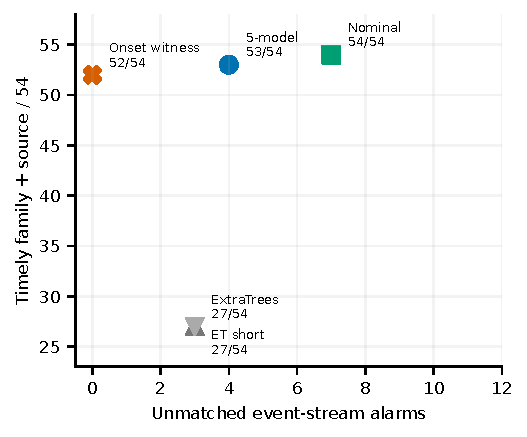
\includegraphics[width=\columnwidth]{figures/generated/narrative_tradeoff.pdf}
\caption{The decision that an accuracy-only table hides. H04 development outcomes trade timely attribution against unmatched event-stream alarms. The onset-witness ablation removes all extras but loses a real BUS16 intervention; it is retained as negative evidence. Labels use 54 paired realizations of 18 interventions and do not imply 54 independent trials.}
\label{fig:narrative-tradeoff}\end{figure}

An additional onset-witness publication ablation reaches zero extras while reducing timely attribution to \ContAdmissionTimely{}/\ContAdmissionTotal{}. It rejects a true BUS16 load with weak early onset evidence. The physical states and underlying masses are inherited, so suppressing the public alarm does not repair the estimator's explanation. We retain this as a negative experiment rather than select it for its zero-extra count. R11 and nominal remain frozen for C01.

\subsection{What Is Still Being Confirmed}

The present development evidence supports causal load/line attribution on a known catalog and shows its failure modes. It does not yet support a final performance claim on C01. The confirmatory executor is running with fixed methods, cases, thresholds and metrics; its completed results will enter the dedicated section below through the same hash-to-table/figure chain. No partial C01 result is used here to choose a variant or revise the method.

\clearpage
\begin{figure*}[p]\centering
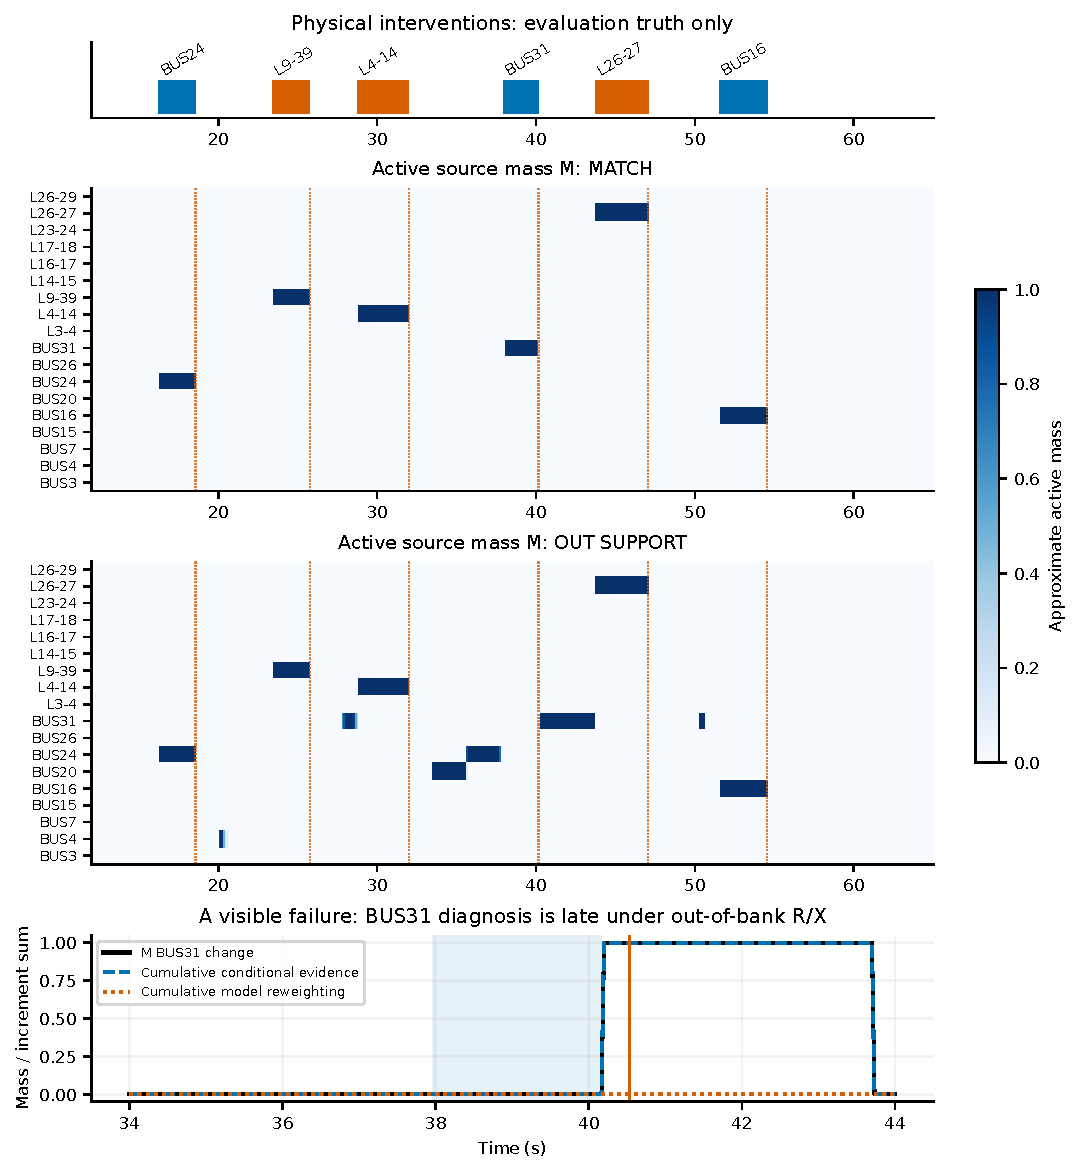
\includegraphics[width=.95\textwidth]{figures/generated/narrative_rolling.pdf}
\caption{From a sequence to an attribution array. Top: reserved physical intervention intervals in fixed H04 parent H002. Middle: causal active masses across the 18 admissible cells for paired nominal and out-of-bank records. Orange dotted lines mark true OFF for evaluation only. Bottom: BUS31 under out-of-bank R/X, with the exact cumulative decomposition of $\Delta M$ relative to 34 s into conditional evidence and model reweighting. The diagnosis marker is later than OFF: an eventual correct source is not a timely success. This is a development illustration, not C01 confirmation or a calibrated probability display.}
\label{fig:narrative-rolling}\end{figure*}
\clearpage

\IfFileExists{sections/08c_c01_confirmatory.tex}{\input{sections/08c_c01_confirmatory}\FloatBarrier}{}
\section{Interpretation and Limits}
\label{sec:discussion}

The bank constructs each candidate from the network equations rather than fitting a source-label decision boundary. That is an architectural distinction, not evidence of causal source-excluded generalization. It retains the explanation as states evolve and distinguishes an operator being restored from the grid returning to equilibrium. In this development test the practical gain is timely load attribution; line attribution does not separate the physical and learned references.

That conclusion has three boundaries. First, the causal result uses a known nine-load/nine-line catalog and an intervention-free startup. It is not a test of all 39 buses or arbitrary unknown event families. Second, the instrument and terminal map are frozen research assumptions, including the provisional BUS5 assignment and excluded BUS39 current angle. Agreement within that model does not establish the producer's actual CT placement or exact replication of RAW0001. Third, the network bank is finite and its startup nuisance estimates are plug-in. Its masses are useful attribution weights but are not demonstrated calibrated probabilities.

The nominal reference and failed onset-witness ablation prevent a stronger accuracy claim. More network hypotheses reduce extras in H04 but delay a BUS31 decision; more restrictive admission removes extras but rejects a real BUS16 event. Those are differences in what the decision retains and when it is emitted. Reporting eventual source recovery, or zero extras alone, would select different winners and hide the trade-off.

The mathematical interpretation is equally scoped. Good hidden-voltage reconstruction does not prove event separability. The batch test supports the importance of profiled response overlap, but does not validate every analytic small-amplitude or changing-sensor limit in the supplement. The 137-support batch reference retains its original quadrature; the causal implementation has not been proved to be the unrestricted joint estimator or an exact reduction of it.

The ExtraTrees result tests the particular frozen causal adapters under these physical conditions. Their load failure calls for that restricted interpretation, rather than a general statement that ML cannot recognize loads. Likewise, Chen's colored-noise/DC mismatch is kept visible instead of being used to claim universal superiority over the published algorithm under its own assumptions.

The closest-method comparison narrows the novelty claim further. Warner's
trajectory scan already supplies physical transient signatures, unknown-onset
search and sparse remote sensing; the Adaptive Matrix CuSum supplies
sequential diagnosis theory. Our evaluated construction addresses a different
operational target: successive load/line histories whose restoration and
electrical recovery are distinct. The present evidence does not establish
superiority over those unexecuted comparators or a false-alarm guarantee.
Nor does the component-level source geometry yet provide a calibrated
online abstention certificate for R11.

A physics-informed extension should preserve this distinction rather than
merely add a learned label head. Physics-derived stochastic priors can
propagate uncertainty in unmeasured forcing \cite{ensaf2023kernel,tartakovsky2023gp},
while joint DAE parameter inference addresses a different identification
problem \cite{albustami2026dae}. A future discrepancy model would have to
separate such uncertainty from intervention signatures and instrumental
noise. That is a new validation question, not a feature silently added to
the frozen C01 method or a condition introduced to postpone this paper's closure.

The final decision rests on the prespecified C01 comparison and claim/evidence review, without another bus-specific correction. Faults, generation mechanisms, PMU loss, unseen-source causal transfer and field operation are future scopes, not hidden requirements for reporting this restricted result. The proposed joint estimator remains documented in the supplement so that exploratory work is preserved without being mistaken for the mechanism validated here.

\section{Conclusion}
\label{sec:conclusion}

The contribution is a recovery-aware physical attribution construction for sparse PMUs: a restored operator leaves a dynamic state that continues to explain measurements and must compete with later interventions. The implemented load/line bank predicts intervention-conditioned DAE histories and mixes fixed network hypotheses. $M$ records the source masses; $\Delta M$ separates within-model evolution from model reweighting. Physical templates and unknown-onset scans have close precedents, and this study does not establish superiority over unexecuted trajectory-based methods.

The completed development evidence shows both utility and a limit. Physical state recovery can be accurate while weak event sources remain ambiguous. In causal H04 development, the five-model reference obtains \ContMixTimely{}/\ContMixTotal{} timely joint decisions with \ContMixExtras{} extras; nominal improves timeliness at a higher alarm burden. The family and temporal breakdowns explain that result, including the BUS31 delay and the negative BUS16 admission experiment. Final performance claims depend on the frozen confirmatory results. No broader all-family, unseen-source or field claim follows from these tests.

\section*{Supplementary Material}
The supplement preserves detailed proofs, electrical and instrumental conventions, the original batch estimator and joint-estimator proposals, expanded component studies, and complete evidence contracts. The pre-revision manuscript is archived in the repository. Empirical data and inference baselines are unchanged.


% Acknowledgments and author biographies are intentionally omitted until author-provided.
\FloatBarrier
\bibliographystyle{IEEEtran}
\bibliography{references}

\EOD
\clearpage
\IfFileExists{\PSevenSupplementPDF}{%
  \includepdf[
    pages=-,
    fitpaper=true,
    pagecommand={\thispagestyle{empty}},
    addtotoc={1,section,1,{Supplementary Material},supplementary-material}
  ]{\PSevenSupplementPDF}%
}{%
  \PackageError{P07}{Supplementary PDF not found}{Run scripts/build_manuscript_bundle.ps1 before compiling main.tex.}%
}
\end{document}
